\chapter{Implementation}
\label{cha:implementation}

The system is realized through a local network of Docker instances, each running a microservice needed for the purpose of evaluated the system at the users that view the videos. This network has multiple services which are described in \autoref{sec:impl-overview}
One of these components are the clients watching the video. Whose view patterns are determined by their persona, which are described in \autoref{sec:impl-personas}.
For the users to watch the videos they had to be processed into a \ac{DASH} format suited for streaming, how this is implemented is presented in \autoref{sec:impl-video}.
Then the setup for the experiment is presented in two parts. First the tools that are used (\autoref{sec:impl-setup}) and second the sequence of the individual steps that are performed during the experiments (\autoref{sec:impl-flow}) including how the network is initialized, how data is extracted and more.

\section{Overview}
\label{sec:impl-overview}
The system  contains multiple microservices realized in a docker network:

\begin{itemize}
    \item \texttt{bootstrap} runs an \ac{IPFS} daemon and is responsible for initializing the \ac{IPFS} network, all other participants in the network connect through this node. 
    The Go implementation of \ac{IPFS} (go-ipfs\footnote{\url{https://github.com/ipfs/go-ipfs}}) is used as back-end instead the JavaScript implementation, due to performance. This is due to the goal being performance measurings, where Go should perform better. The go-ipfs must run as a daemon in the background. This is tolerable, due to the vision of having \ac{IPFS} implemented and running natively in the browser.
    \item \texttt{client} represents the users of the system, and there can be arbitrarily many of them depending on the test. The clients run an \ac{IPFS} daemon and a browser that is controlled through Splinter, they then play various videos hosted in the network through the \ac{IPFS} \ac{API} from the \texttt{dash.js} video player with different viewing patterns and connection conditions.
    \item \texttt{host} hosts the \ac{HTML} website that the dash.js player resides on, each client could host this themselves, but having it a single place makes the system more mutable.
    \item \texttt{metric} is a client to the Mongo database that is contacted by the client, the clients reguarly report data regarding their viewing session to Metric which then forwards this to the database, this data includes latency for getting a segment, whether the video stalled and more.
    \item \texttt{network} accesses the docker \ac{API} to get network stats for all the clients, these stats are then stored in the database
    \item \texttt{mongo} is a dockerized Mongo database.
    \item \texttt{plot} is a Mongo client that processes the data stored in the Mongo database and presents it with various plots, it can also export this to a \ac{CSV} format.
    \item \texttt{pumba} is a chaos engineering tool that is used to manipulate the \texttt{client} instances in terms of their download and upload speed, latency and even shutting them down. While \texttt{pumba} could be use as a container, it's opted to use as a binary for ease of automation. 
\end{itemize}
Relation between these services is also illustrated in \autoref{fig:uml_docker-compose}.

\begin{figure}[bth]
    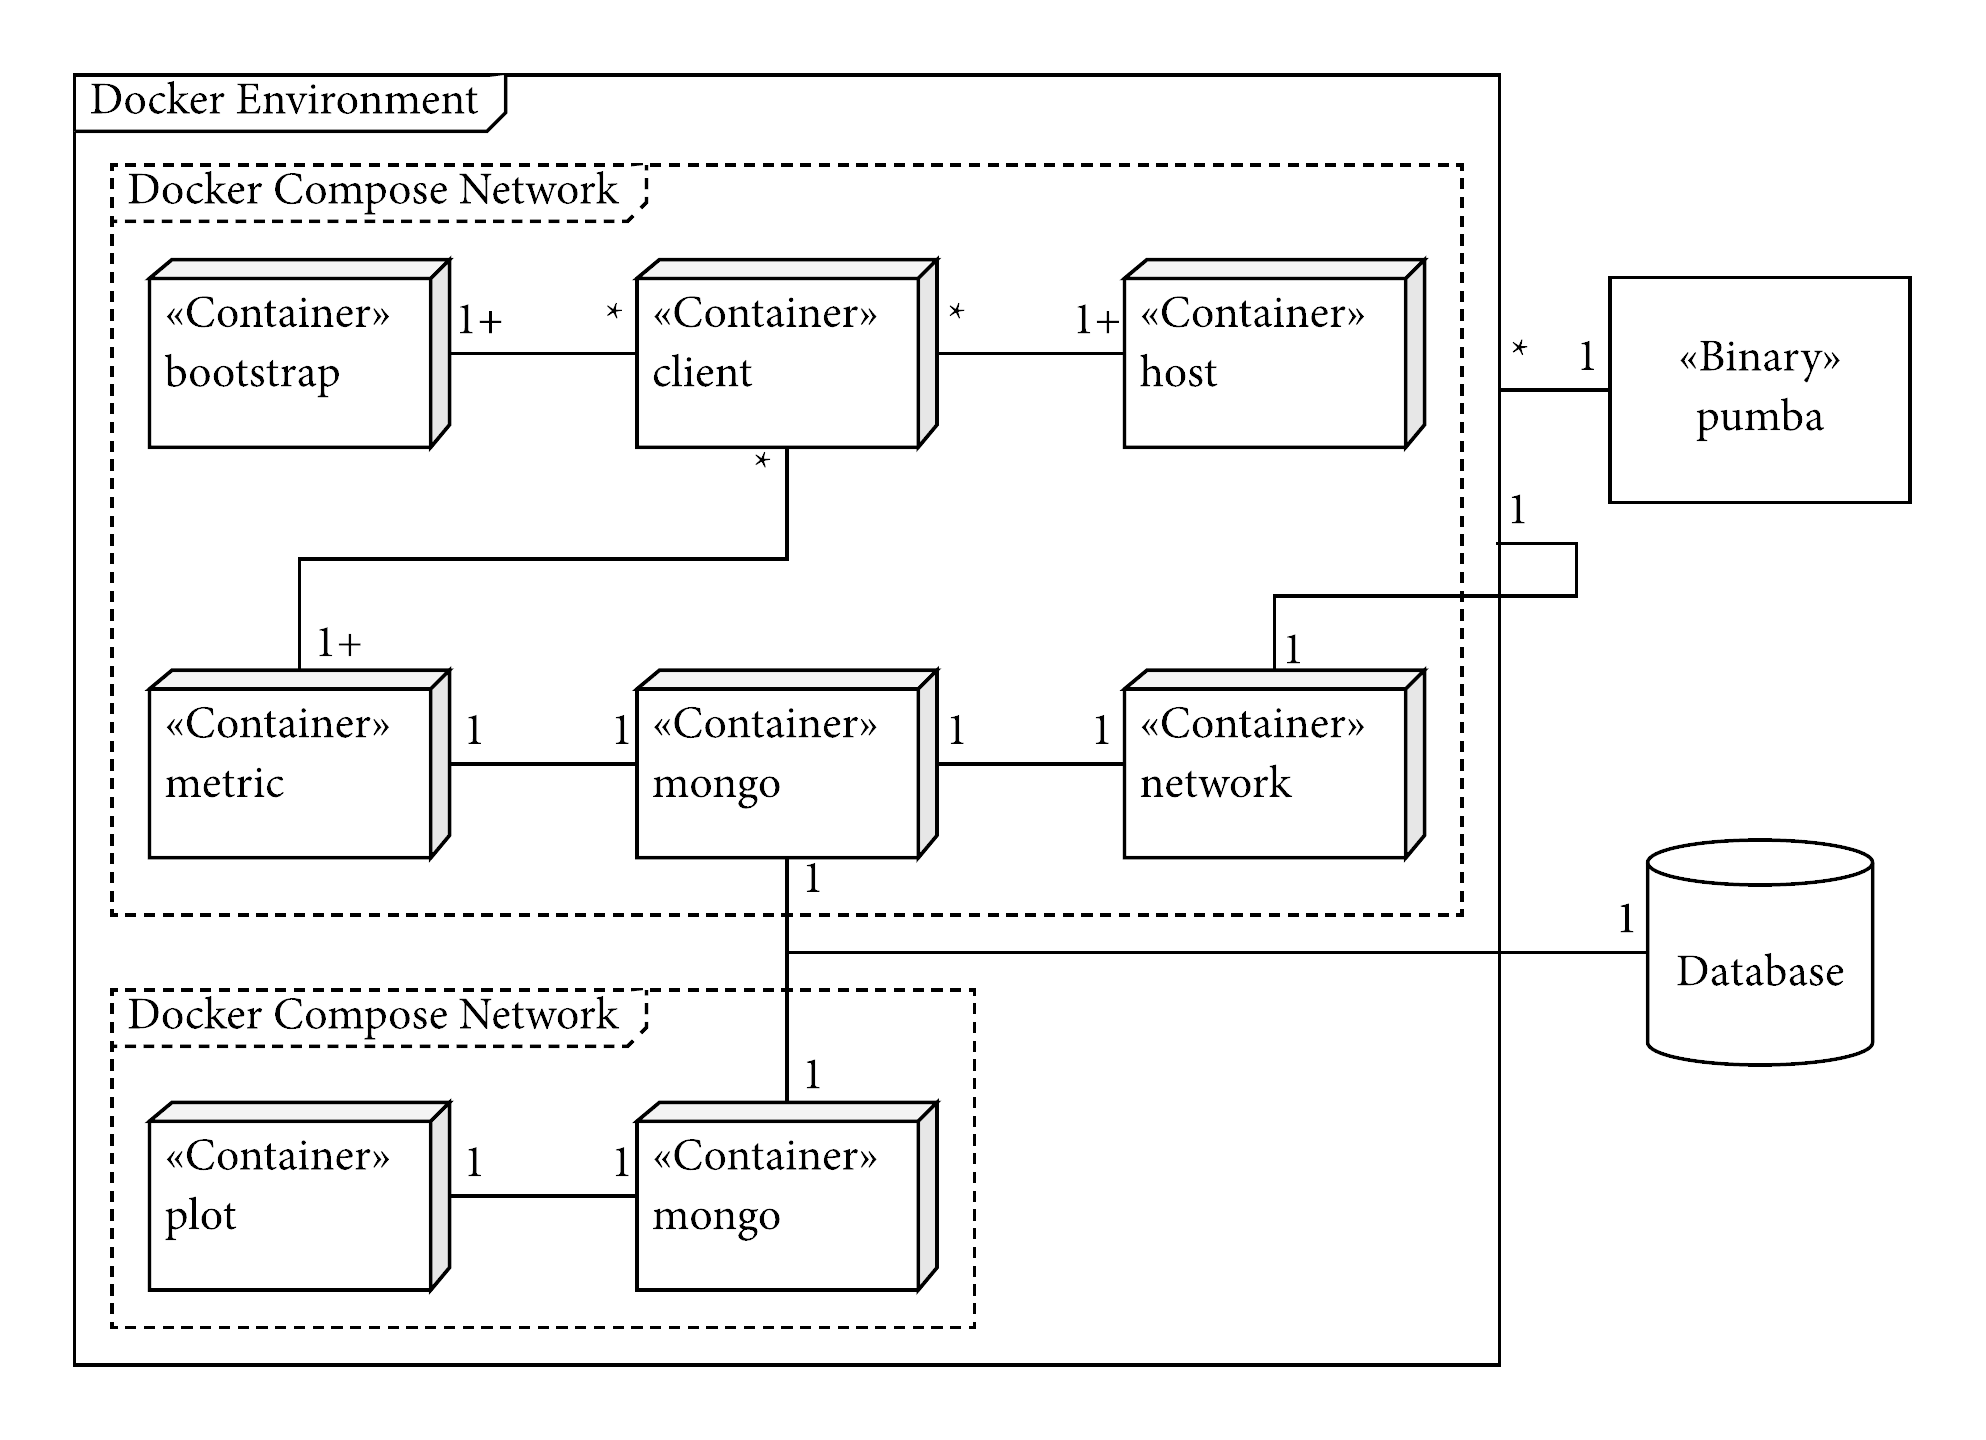
\includegraphics[width=\textwidth]{UML/uml_docker_setup_v95.png}
    \caption[Diagram of the experimental test  setup]{Diagram of the experimental test setup, illustrating the relations between the Docker containers described in \autoref{sec:impl-overview}.}
    \label{fig:uml_docker-compose}
\end{figure}

\section{Personas}
\label{sec:impl-personas}
The clients viewing patterns are determined by their persona, the different types of personas are described in \autoref{sec:individual-behavious}, in these section how these personas are realised will be described.
All personas function by giving them a hash that functions as a path to an \ac{MPD} file
\begin{itemize}
    \item \texttt{Idle} simply does nothing actively, but instead just participates in the network, which is implemented by having the client sleep, while the \ac{IPFS} daemon runs in the background.
    \item \texttt{Seeder} behaves like a Idle persona, but stores the video that the other peers request. When the seeder is started it immediatly adds the video files to the network.
    \item \texttt{Binger} uses splinter to view the video for the \ac{MPD} file, this is done through its local \ac{IPFS} gateway thereby forcing the \ac{IPFS} client to retrieve the video and store it in the peer. The data is not pinned, meaning that if the assigned storage runs out the video data will eventually be deleted.
    \item \texttt{Leecher} behaves like the binge persona but instead of using its own local \ac{IPFS} gateway it uses one of the seeder's instead, this way it can download the video files without using \ac{IPFS} to retrieve them and instead does it through the browser
    \item \texttt{Skipper} is like binge, but instead of viewing the entirety of the video without interacting with it, it watches small segments at a time. By watching a small configurable amount of seconds and then skipping forward another configurable amount of seconds  in the video. This pattern is repeated until the end of the video is reached. This is also illustrated in the pseudocode (\autoref{lst:skipper_pseudo}), where skipLength and watchTime are configurable and timeInVideo, is how far into the video the persona are (in seconds).
    \lstinputlisting[
    language=pseudo,
    caption={Skipper pseudocode},label={lst:skipper_pseudo}]
    {code/skipper.txt}
    \item \texttt{Incognito} is very similar to skipper but instead of watching many segments each a few seconds long. It instead immediatly on startup skips to a configurable amount of seconds before the end of the video, that it watches without any further skips.
\end{itemize}
The remaining Mobile user persona is achieved differently as it is not necessarily a different view pattern but instead different network conditions. Mobile user is then achieved by using one of the above personas but giving it reduced bandwith through Pumba.

\section{Video Content Tools}
\label{sec:impl-video}
Using the Python script \texttt{encode.py}, video content for testing were generated for sharing and streaming in the experimentation. The following tools were used to generate the content.

\subsection{FFmpeg}
The commandline program \texttt{ffmpeg}\footnote{\url{https://ffmpeg.org}} was used for transcoding videos to the proper codecs. The used codecs is chossen to H.264 for video and AAC for audio. 
\texttt{ffmpeg} also makes it possible to change the number of I-frames, which could be necessary due to the segmentation of the streams into multiple files in the DASHing process.

\subsection{MP4Box multimedia packager}
The tool MP4Box from the GPAC framework\footnote{\url{https://github.com/gpac/gpac}} was used to split the streams into segment files and generate a \ac{MPD}.

\subsection{encode.py}
The Python script can take a number of options, in which it, among others, is possible to alter the quality (and thereby bitrate) of the produced video and also set the duration of the segments dashed.

The script operates in 4 steps:
\begin{enumerate}
    \item Encode video and audio to correct media container and codecs using \texttt{ffmpeg}.
    \item Format the newly encoded media container to the wanted DASH profile of specified segment length using \texttt{MP4Box}.
    \item Generate \ac{IPFS} hash addresses of the formatted media using \texttt{ipfs}.
    \item Replace location of segments in \ac{MPD} with hash addresses.
\end{enumerate}

Since the hash addresses always will be the same for the content, it is possible to pre-generate and add the addresses to the \ac{MPD} before any files are shared in \ac{IPFS}, no matter which client latter will add them (See \autoref{sec:ipfs-objects} for more information).

\lstinputlisting[
    language=MPD,
    caption={
        [\acs{MPD} snippet with location addresses]
        Snippet of \ac{MPD} using the location addresses based on file path. For the \ac{MPD} in its entirety, see \autoref{app:mpd}},
    firstnumber=25, 
    firstline=25, 
    lastline=30]{code/dashed.mpd}

\lstinputlisting[
    language=MPD,
    caption={
        [\acs{MPD} snippet with content addresses]
        Snippet of \ac{MPD} using the content addresses based on \ac{IPFS} hashing of file},
    firstnumber=25, 
    firstline=25, 
    lastline=30]{code/hashed.mpd}



\section{Experimentation Setup}
\label{sec:impl-setup}
The following section describes how the experiments were set up, making it possible to recreate the experiments and generated data.


\subsection{\acl{VM}}
\label{sec:setup_vm}
Experimentation is performed on a VMware \ac{VM} with 16 cores\footnote{Intel\textregistered Xeon\textregistered CPU E5-2697A v4 @ 2.60GHz}, 16 GB memory running Ubuntu 16.04\footnote{Ubuntu 16.04.3 LTS (GNU/Linux 4.4.0-104-generic x86\_64)}.


\subsection{Docker}
\label{sec:setup_docker}
\label{sec:setup_docker-compose}
The experimentation is done by emulating clients in a closed network using Docker virtulization. Docker is a tool that can package an application and its dependencies in a virtual \emph{container} that can run on any Linux server. In contrary to \acp{VM}, containers share \ac{OS} and bins/libraries where appropriate, while still being isolated (See \autoref{fig:vm_vs_container}). This results in lower overhead for each instance running, making it possible to easily scale and run more instances on the infrastructure (See \autoref{fig:vm_vs_container}).
The \ac{VM} runs Docker at version 18.03\footnote{Docker CE version 18.03.0-ce, build 0520e24}.

\begin{figure}
    \myfloatalign
    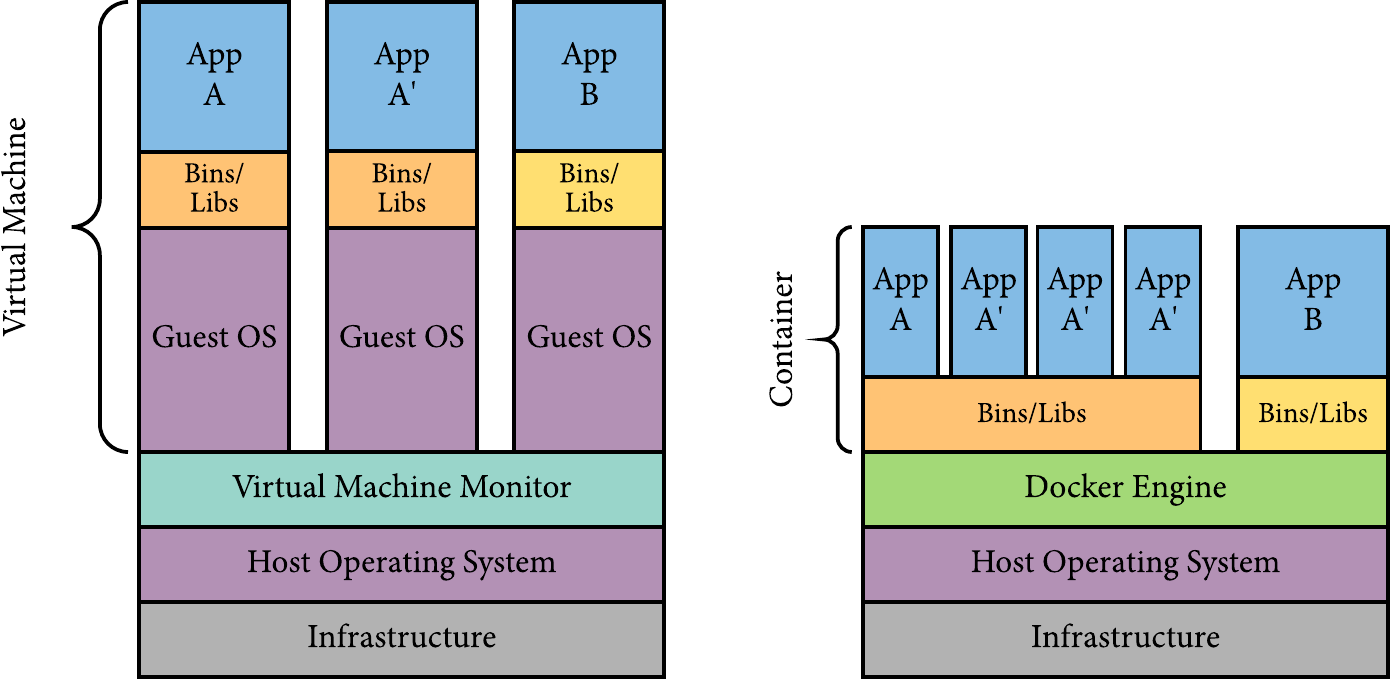
\includegraphics[width=\textwidth]{vm.png}
    \caption[Comparison of \acp{VM} and Docker]{Comparison of the overhead present in virtualization done by \acp{VM} and by Docker}
    \label{fig:vm_vs_container}
\end{figure}

Docker compose is used to orchestra the virtual network and it's containers. This makes it possible to run multi-container applications,  meaning to define a setup with containers being dependant on each other and to start them in the correct order. This is exemplified in the compose file \autoref{lst:compose-example}, line 8-12.

Besides defining dependencies, the compose file is also used for other options. In the case of the Seeder a local directory is mounted, containing the files to be seeded in \ac{IPFS} (See \autoref{lst:compose-example}, line 6-7), so if the service \texttt{user\_seed} was scaled to multiple instances, the video wouldn't need duplication.
Finally the command option defines the client behavior, and the Seeder have the default role of a Seeder persona with 0 seconds start up (See \autoref{lst:compose-example}, line 13), but with the ability to change the behaviour by utilizing an env file containing the variable \texttt{USER\_SEED} defined (See \autoref{lst:env_stable} or \ref{lst:env_exp} for example). 
Docker compose checks on run time if a \emph{.env} file is present in the working directory, and if so, substitutes all defined variables in the compose file. This allows for manipulating the setup at each compose run, by serving docker compose new environment files.

Docker Compose is used on the \ac{VM} at version 1.20.1\footnote{docker-compose version 1.20.1, build 5d8c71b}.

\lstinputlisting[
    language=docker-compose,
    label={lst:compose-example},
    caption={
        [Docker compose file snippet]
        Snippet of a Docker compose file used to define users in the network. Here only the Seeder service (\texttt{user\_seed}) is shown. For full compose file see \autoref{app:compose}.}]{code/compose-example.yml}


\subsection{Pumba}
\label{sec:setup_pumba}
Pumba is a resilience testing tool used to help with the conduction of the experiments. It can manipulate the network condition of docker containers as well as pause and/or stop containers, either chosen randomly or deterministically. Pumba utilizes the Docker \ac{API}\footnote{\url{https://docs.docker.com/engine/api/v1.30/}} for the resilience testing, tc\footnote{traffic control: \url{https://linux.die.net/man/8/tc}} and iproute2\footnote{\url{https://wiki.linuxfoundation.org/networking/iproute2}} for network manipulation. For the experiments to emulate real world network conditions, the network manipulation are the primary focus of this tool.
The \ac{VM} runs pumba at version 0.4.8\footnote{pumba version 0.4.8, build 537d77d}. 

\subsection{IPFS}
\label{sec:setup_ipfs}
The containers run \ac{IPFS} at version 0.4.14\footnote{go-ipfs version 0.4.14, build 5db3846}.


\subsection{dash.js}
\label{sec:setup_dash.js}
The \texttt{website} container uses dash.js\footnote{\url{https://github.com/Dash-Industry-Forum/dash.js/}} at version v2.6.8\footnote{dash.all.min.js version 2.6.8, build 888cdcc4}, which adds the \ac{DASH} compatibility to the \ac{HTML}5 video player using JavaScript, which is needed to accomplice the intended design.
The chosen format for the stream is selected from the DASH-AVC/264 standard\cite{dash264}, due to its interoperability and because it's supported by the \texttt{dash.js} player.
The standard defines the multimedia container as MP4, the video codec as H.264 and the audio codec as AAC. As a addition separate audio and video streams are required, which means that multiplexing isn't allowed.
Dash.js manages retrieving of video and audio segments by itself, and no other segment retrieval techniques are implemented. Note audio and video are separated into two different tracks of segments for dash.js to be able to play the video.

\subsection{Python \& Splinter}
\label{sec:setup_python}
\label{sec:setup_splinter}
The containers run Python at version 3.5.2, for running the entrypoints (See \autoref{sec:setup_docker}) of the containers.

Splinter\footnote{\url{https://github.com/cobrateam/splinter}} is a Python library used for emulating user input through a browser. Various personas (See \autoref{sec:individual-behavious}) will be interacting with the website through a chrome browser (at version 64.0\footnote{Google Chrome version 64.0.3282.140 (Official Build) (64-bit)}) by utilizing this library, and thereby emulating different behaviours.
The package splinter used is at version 0.7.7.


\section{Experiment flow}
\label{sec:impl-flow}
Experiments are first started by setting up a stable network of the required services for the experiment. This stable setup is given an initialization time to ensure it's stabilized, meaning that an \ac{IPFS} network has formed and seeders have added their files to the network.
After a configurable delay the clients are added to the network, and start performing the actions that their persona and the entrypoint program describes (As described in \autoref{sec:experiment_entrypoint} and \autoref{fig:entrypoint_sequence}).
The experiment then runs for a configurable amount of time that should give enough time for all clients to finish viewing the video. When the time is up every microservice is terminated and the plot service is started to graph the collected from the experiment (As seen in \autoref{fig:run_sequence_plot}).

The orchestration of this is handled by the run script \texttt{run.py}, as described in the following \autoref{sec:experiment_run} and can be seen in the sequence diagrams; \autoref{fig:run_sequence_clean}, \ref{fig:run_sequence_exp} and \ref{fig:run_sequence_plot}.

\subsection{Experimental Environments}
\label{sec:experiment_env}
Each experiment is designed by creating two environment files, describing which services should run, which options should they run with and how many instances shall be created. The reason two environment files is needed is that one defines the stable network and the other defines the clients add for the experiment. An example of a environment files can be seen at \autoref{lst:env_stable} and \ref{lst:env_exp}.

\noindent\begin{minipage}[t]{.35\textwidth}
\lstinputlisting[language=env,
                 caption={Stable env file},
                 label={lst:env_stable}]
                {code/env_stable.env}
\end{minipage}
\hfill
\begin{minipage}[t]{.52\textwidth}
\lstinputlisting[language=env,
                 caption={Experiment env file},
                 label={lst:env_exp}]
                {code/env_exp.env}
\end{minipage}\bigskip

The experiments are run with a default stable network which includes one instance of every role listed in \autoref{sec:impl-overview} except \texttt{client} and \texttt{plot}, which is handled differently. The \texttt{client}s are initialized based on their persona, and only the seeder personas are added to the stable part of the network.
The seeder holds the \ac{MPD} file as well as the video segments in the \ac{IPFS} network, for the other users to retrieve. 

\subsection{run.py}
\label{sec:experiment_run}
The experiments are executed using the the script \texttt{run.py}, which takes the two environment files (See \autoref{sec:experiment_env}) as arguments. The run script consists of 3 overall stages.

The first stage consists of the database being dropped, should there be any data left from a previous or failed experiment (See \autoref{fig:run_sequence_clean}). This is done by running the \texttt{mongo} service solely, followed by an docker-compose exec command which runs mongo shell command, dropping the database. This have to be done, due to the data being stored on the host machine of Docker, to easy access and ensure persistence. Since the \texttt{mongo} service needs time to start before the command can be executed, we have to try multiple times until  we receive a correct return code. Afterwards all services are killed, to stop the mongo instance, avoid other hanging services interference and ensure a fresh start for the new experiment. This stage is also run at the end of each experiment.


\begin{figure}
    \centering\footnotesize\sffamily
    \caption[Sequence diagram for run script pre-processing]{Sequence diagram of run script pre-processing, illustrating the clean up run at the beginning and end of each experiment}
    \label{fig:run_sequence_clean}
    \begin{sequencediagram}
    \newthread{run}{\normalsize Run.py}
    \newinst[1]{dc}{\normalsize Docker compose}
    \newinst[1]{doc}{\normalsize Docker}
    
    \begin{call}{run}{\shortstack{run \textit{mongo}}}{dc}{}
        \begin{messcall}{dc}{run \textit{mongo}}{doc}{}
            \begin{sdblock}{loop}{Until exit 0}
                \begin{call}{dc}{exec drop db}{doc}{}
                \end{call}
            \end{sdblock}
        \end{messcall}
    \end{call}
    
    \begin{messcall}{run}{down}{dc}{}
        \begin{messcall}{dc}{kill \textit{all containers}}{doc}{}
        \end{messcall}
    \end{messcall}
    
    \end{sequencediagram}
\end{figure}

The second stage consists of the set up of the stable network, followed by the experiment after it's stabilization (See \autoref{fig:run_sequence_exp}). First the scales defined in the environment file for the stable network are extracted. The scales are needed by \texttt{run.py}, since the scaling is done through the \ac{CLI} of docker-compose's up command, which have a scale option \footnote{\url{https://docs.docker.com/compose/reference/up/}}. As default \textit{run.py} sets the scale of all services to 0, which is then overwritten by environmental files in two sittings.
After importing the scales, the environmental file as soft linked to \texttt{.env}, which is as an environment for the compose file used by docker-compose\footnote{\url{https://docs.docker.com/compose/env-file/}}.
The user behaviours from the environment file is then used along with the compose file by docker-compose when calling the run command on docker.
When the scaling of the stable network have begun, \textit{run.py} busy waits for a configurable amount of time until all services are running and are stabilized, which is based on empirical data from the \ac{VM}.
After the stabilization the \textit{clients} are added to measure their influence on the network and their individual \ac{UX}. This is mainly done with the same procedure as the stable network, but from another environment file. The only difference in the procedure are pumba (See \autoref{sec:framework_pumba}
 and \ref{sec:setup_pumba}) is run to influence the network for all clients, before busy waiting for the length of the experiment.
Finally all services are killed, to stop the data collection of the experiment.

\begin{figure}
    \centering\footnotesize\sffamily
    \caption[Sequence diagram for run script (2/3)]{Sequence diagram of run script (Part 2 of 3), illustrating the setup of a stable network and the execution of an experiment.}
    \label{fig:run_sequence_exp}
    \begin{sequencediagram}
    \newthread{run}{\normalsize Run.py}
    \newinst[3]{dc}{\normalsize Docker compose}
    \newinst[1]{doc}{\normalsize Docker}
    \newinst[1]{pum}{\normalsize Pumba}
        
    \begin{call}{run}{extract scales from \textit{stable} env file}{run}{}
    \end{call}
    
    \begin{messcall}{run}{set \textit{stable} env file as environment}{dc}{}
    \end{messcall}
    
    \begin{messcall}{run}{scale \textit{stable service(s)}}{dc}{}
        \begin{sdblock}{loop}{\shortstack{Iterate through services and scale\\according to  the \textit{stable} env}}\postlevel
            \begin{messcall}{dc}{run \textit{stable image}}{doc}{}
            \end{messcall}
        \end{sdblock}
    \end{messcall}
    
    \begin{call}{run}{busy wait until network is stabilized}{run}{}
    \end{call}
    
    \begin{call}{run}{extract scales from \textit{exp} env file}{run}{}
    \end{call}
    
    \begin{messcall}{run}{set \textit{exp} env file as environment}{dc}{}
    \end{messcall}
    
    \begin{messcall}{run}{scale \textit{exp service(s)}}{dc}{}
        \begin{sdblock}{loop}{\shortstack{Iterate through services and scale\\ additionally with scales from \textit{exp} env}}\postlevel
            \begin{messcall}{dc}{run \textit{exp image}}{doc}{}
            \end{messcall}
        \end{sdblock}
    \end{messcall}
    
    \begin{messcall}{run}{Manipulate network for all \textit{users}}{pum}{}
        \begin{call}{pum}{adjust network}{doc}{}
        \end{call}
        \begin{call}{run}{busy wait for chosen length of experiment}{run}{}
        \end{call}
    \end{messcall}
    
    \begin{messcall}{run}{down}{dc}{}
        \begin{messcall}{dc}{kill \textit{all}}{doc}{}
        \end{messcall}
    \end{messcall}
    
    \end{sequencediagram}
\end{figure}

The third stage consists of plotting the results and export the data to an archive (See \autoref{fig:run_sequence_plot}). Since plot isn't a part of the experiment it's defined in a separate compose file (\textit{plot-compose.yml}), which is used with docker compose to generate the plots. Since the data is kept in a mongoDB, the \texttt{plot} service is dependent on the \texttt{mongo} service. This effectively means that when docker compose is asked to run the \texttt{plot} service, the dependencies is also started. Since \texttt{plot} terminates when all plots are done, we wait for it to exit before continuing.

After the termination of \texttt{plot}, the data from the still present \texttt{mongo} service is exported to a gzip\footnote{\url{https://www.gnu.org/software/gzip/}} archive using the utility mongodump\footnote{\url{https://docs.mongodb.com/manual/reference/program/mongodump/}}. 


\begin{figure}
    \centering\footnotesize\sffamily
    \caption[Sequence diagram for run script (3/3)]{Sequence diagram of run script (Part 3 of 3), illustrating the plotting and export of data at the end of each experiment}
    \label{fig:run_sequence_plot}
    \begin{sequencediagram}
    \newthread{run}{\normalsize Run.py}
    \newinst[1]{dc}{\normalsize Docker compose}
    \newinst[1]{doc}{\normalsize Docker}
    
    \begin{call}{run}{run \textit{plot}}{dc}{}
        \begin{messcall}{dc}{run \textit{mongo}}{doc}{}
            \begin{call}{dc}{run \textit{plot}}{doc}{plots generated}
            \end{call}
        \end{messcall}
    \end{call}
    
    \begin{call}{run}{export data}{dc}{}
        \begin{call}{dc}{exec mongodump}{doc}{store gzip of db}
        \end{call}
    \end{call}
    
    \end{sequencediagram}
\end{figure}

\subsection{entrypoint}
\label{sec:experiment_entrypoint}

The entrypoint is illustrated in \autoref{fig:entrypoint_sequence} the client starts by performing the initialization of the \ac{IPFS} peer, here the peer solves a crypto-puzzle in order to generate a peer id, and key-pairs used for secure communication.
Next the client starts a local daemon and connects to the peers listed in it's list of bootstrap peers, which can either be ones limited to a small network entirely for the experiment or the bootstrap peers that one would use to connect to the global \ac{IPFS} network.
Starting a daemon also starts a new thread that handles \ac{IPFS} related requests, these are not illustrated in the figure. In order to preserve clarity. These two \ac{IPFS} \ac{API} calls are not performed by the clients with the entrypoint persona, as they do not need it to retrieve the video segments.\\
The client then launches a Google Chrome\footnote{\url{https://www.google.com/chrome/}} browser that is controlled through Splinter and requests the website containing the video player from the Host container, the website is stored in a separate container to ease modifications during development.
After receiving the website, Splinter starts the video player, which requests the \ac{MPD} file, from other peers in the \ac{IPFS} network, through its own gateway, or the seeder's in the case of the leecher.
After receiving the \ac{MPD} the video can start and persona behaviour is then performed. While watching the video the client requests the necessary segments as it needs them until all segments have been received.
When the video is finished the browser is then closed and the client either starts busy waiting or terminates. If the client busy waits the daemon thread is kept alive meaning other peers can retrieve data from the client.\\

\begin{figure}
    \centering\footnotesize\sffamily
    \caption[Sequence diagram for clients]{Sequence diagram of client requesting video pieces in the \acs{IPFS} network}
    \label{fig:entrypoint_sequence}
    \begin{sequencediagram}
        \newthread{p1}{\normalsize Client}
        \newinst[4]{p2}{\normalsize IPFS gateway}
        \newinst[1]{p3}{\normalsize Host}
        \begin{sdblock}{optional}{Leecher does not run IPFS}
            \begin{call}{p1}{IPFS init}{p1}{}
            \end{call}
            \begin{call}{p1}{IPFS Daemon}{p1}{}
            \end{call}
        \end{sdblock}
        \begin{call}{p1}{launch browser}{p1}{}
        \end{call}
        \begin{messcall}{p1}{request website}{p3}
            \begin{messcall}{p3}{send website}{p1}
            \end{messcall}
        \end{messcall}
        \begin{call}{p1}{start video player}{p1}{}
        \end{call}
        \begin{messcall}{p1}{request MPD file}{p2}
            \begin{messcall}{p2}{send MPD file}{p1}
            \end{messcall}
        \end{messcall}
        \begin{sdblock}{loop}{}
            \begin{messcall}{p1}{request segment}{p2}
                \begin{messcall}{p2}{send segment}{p1}
                \end{messcall}
            \end{messcall}
        \end{sdblock}
        \begin{sdblock}{loop}{}
            \begin{call}{p1}{busy wait}{p1}{}
            \end{call}
        \end{sdblock}
    \end{sequencediagram}
\end{figure}

\section{Summary of Implementation}
The realized system contains multiple components, first of there is the Personas that specify how a client acts after video playback has started, these come in multiple varieties.
\begin{itemize}
    \item The Seeder shares files.
    \item The Binger watches video, without any interaction.
    \item The Leecher watches video through the Seeders \ac{IPFS} gateway.
    \item The Skipper watches the video but skips forward every couple seconds.
    \item The Incognito user skips to the end of the video.
    \item The mobile user has lower bandwidth, which is realized with Pumba.
\end{itemize}
For the client to be able to watch the videos the need to be encoded. This is done with a combination of \texttt{FFmpeg} and \texttt{MP4Box}. This is done so that the video is in a \ac{DASH} format suitable for streaming.

The testing setup consists of a local network of \texttt{Docker} \acp{VM}, where network conditions is throttled by Pumba, each client hosts \ac{IPFS} and watches the video using the \texttt{dash.js} library, where the user actions can be manged through the \texttt{Splinter} library.

Experiments are run by setting up a stable network first which has necessary microservices needed for the test to work, such as database and file hosting. Afterwards the clients are added and testing begins for a duration, when this passes all clients shut down and plots from the experiments are generated and the database is exported.
% personas
% tools
% setup
% experiment
%%% Local Variables:
%%% mode: latex
%%% TeX-master: "../ClassicThesis"
%%% End:
